
\renewcommand{\arraystretch}{1.8}
\footnotesize
\begin{table}[h]
    \centering
    \footnotesize
    \begin{tabular}
        {
            |>{\centering\hspace{0pt}}m{0.140\linewidth}
            |>{\hspace{0pt}}m{0.300\linewidth}
            |>{\centering\hspace{0pt}}m{0.140\linewidth}
            |>{\hspace{0pt}}m{0.300\linewidth}|
        } 
    \hline
    \multicolumn{4}{|c|}{{\cellcolor{maize}}{\Large\textbf{화 면 정 의 서}}} \\ 
    \hline
    시스템명 & TeulDa & 작성일 & 2021.1.10 \\ 
    \hline
    업 무 명 & 메인 화면 & 작성자 & 왕밤빵 \\ 
    \hline
    화면 ID & Main.jsp & 화면명 & Main \\ 
    \hline
    화면개요 & \multicolumn{3}{l|}{메인 화면} \\ 
    \hline
    \multicolumn{4}{|c|}{}\\
    \multicolumn{4}{|l|}{\textbf{1. 화면 레이아웃}} \\ 
    \multicolumn{4}{|c|}{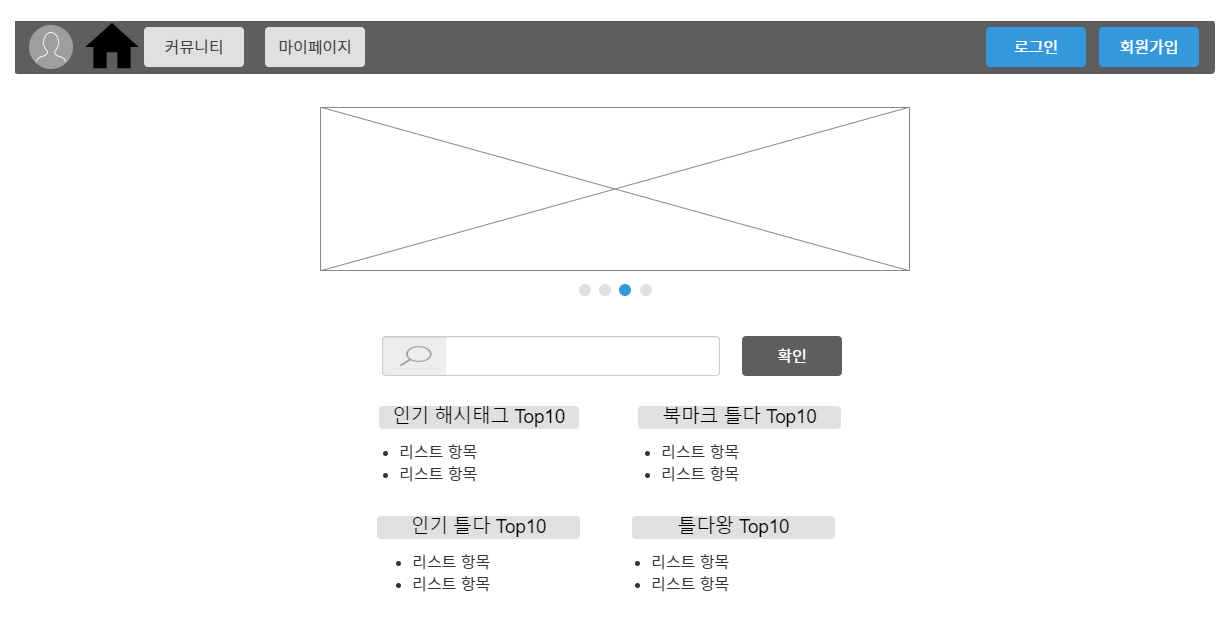
\includegraphics[width=17.00cm]{./Figure/Analysis/Display/main.png}} \\
    \hline
    \end{tabular}
\end{table}

\textbf{2. 데이터 구성 항목}

\begin{longtable}
    {
        |>{\centering\hspace{0pt}}m{0.150\linewidth}
        |>{\centering\hspace{0pt}}m{0.180\linewidth}
        |>{\centering\hspace{0pt}}m{0.060\linewidth}
        |>{\centering\hspace{0pt}}m{0.110\linewidth}
        |>{\centering\hspace{0pt}}m{0.150\linewidth}
        |>{\centering\arraybackslash\hspace{0pt}}m{0.190\linewidth}|
    } 
    \hline
    \rowcolor{maize} 항목명(한글) & 컨트롤(영문) & 필수 & 수정여부 & 설명 & 비고/제약사항 \endfirsthead 
    \hline
    검색어 & searchKeyword & Y & Y & 검색어 입력
    & \multicolumn{1}{>{\hspace{0pt}}m{0.190\linewidth}|}{} \\
    \hline
\end{longtable}

\textbf{3. 처리 로직}

\arrayrulecolor{black}
\begin{longtable}
    {
        |>{\hspace{0pt}}m{0.200\linewidth}
        |>{\hspace{0pt}}m{0.150\linewidth}
        |>{\hspace{0pt}}m{0.300\linewidth}
        |>{\hspace{0pt}}m{0.150\linewidth}
        |>{\hspace{0pt}}m{0.200\linewidth}|} 
    \hline
    \rowcolor{maize} 
    \multicolumn{1}{
        |>{\centering\hspace{0pt}}m{0.200\linewidth}|}{{\cellcolor{maize}}} 
        & \multicolumn{1}{>{\centering\hspace{0pt}}m{0.150\linewidth}|}{입력값/파라미터} 
        & \multicolumn{1}{>{\centering\hspace{0pt}}m{0.300\linewidth}|}{처리내용} 
        & \multicolumn{1}{>{\centering\hspace{0pt}}m{0.150\linewidth}|}{출력/처리결과} 
        & \multicolumn{1}{>{\centering\arraybackslash\hspace{0pt}}m{0.038\linewidth}|}{{\cellcolor{maize}}} \\* 
    \hhline{|>{\arrayrulecolor{maize}}->{\arrayrulecolor{black}}|--->{\arrayrulecolor{maize}}->{\arrayrulecolor{black}}|}
    \rowcolor{maize} \multicolumn{1}{
        |>{\Centering\hspace{0pt}}m{0.200\linewidth}|}{\multirow{-2}{0.200\linewidth}{\hspace{0pt}{\cellcolor{maize}}\Centering{}이벤트명}} 
        & \multicolumn{1}{>{\Centering\hspace{0pt}}m{0.150\linewidth}|}{시작 JSP} 
        & \multicolumn{1}{>{\Centering\hspace{0pt}}m{0.300\linewidth}|}{프리젠테이션 레이어 설계} 
        & \multicolumn{1}{>{\Centering\hspace{0pt}}m{0.150\linewidth}|}{출력 JSP} 
        & \multicolumn{1}{>{\Centering\hspace{0pt}}m{0.200\linewidth}|}{\multirow{-2}{0.038\linewidth}{\hspace{0pt}{\cellcolor{maize}}\Centering{}비고}} \\* 
    \hline
    % \multirow{4}{0.255\linewidth}{\hspace{0pt}확인.onClick()} & 검색어 & \multirow{2}{0.347\linewidth}{\hspace{0pt}입력값으로 검색한 결과 화면을 보여준다.} & 검색 결과 화면 이동 &  \\* 
    % \arrayrulecolor[rgb]{0.8,0.8,0.8}\cline{2-2}\arrayrulecolor{black}\cline{4-4}
    %  &  &  &  &  \\* 
    % \arrayrulecolor{black}\cline{2-5}
    %  & Main.jsp & Path : /community/getAll : GET & \multirow{2}{0.129\linewidth}{\hspace{0pt}totalSearch.jsp} &  \\* 
    % \arrayrulecolor[rgb]{0.8,0.8,0.8}\cline{2-2}\arrayrulecolor{black}\cline{3-3}
    %  &  & Controller : com.teulda.web.community.communityController.getAll() &  &  \\* 
    % \arrayrulecolor{black}\hline
    % \multirow{4}{0.255\linewidth}{\hspace{0pt}인기 해시태그 Top10 리스트 항목 중 한개.onClick()} & 검색어(해시태그) & \multirow{2}{0.347\linewidth}{\hspace{0pt}입력값(해시태그)으로 검색한 화면을 보여준다.} & 검색 결과 화면 이동 &  \\* 
    % \arrayrulecolor{black}\cline{2-2}\cline{4-4}
    %  &  &  &  &  \\* 
    % \arrayrulecolor{black}\cline{2-5}
    %  & Main.jsp & Path : /community/getAll : GET & \multirow{2}{0.129\linewidth}{\hspace{0pt}totalSearch.jsp} & \multirow{2}{0.038\linewidth}{\hspace{0pt}} \\* 
    % \arrayrulecolor[rgb]{0.8,0.8,0.8}\cline{2-2}\arrayrulecolor{black}\cline{3-3}
    %  &  & Controller : com.teulda.web.community.communityController.getAll() &  &  \\* 
    % \arrayrulecolor{black}\hline
    % \multirow{4}{0.255\linewidth}{\hspace{0pt}북마크 틀다 Top10 리스트 항목 중 한개.onClick()} & 기록번호 & \multirow{2}{0.347\linewidth}{\hspace{0pt}기록번호와 일치하는 기록 상세조회 화면을 보여준다.} & 기록 상세조회 화면 이동 &  \\* 
    % \arrayrulecolor[rgb]{0.8,0.8,0.8}\cline{2-2}\arrayrulecolor{black}\cline{4-4}
    %  &  &  &  &  \\* 
    % \arrayrulecolor{black}\cline{2-5}
    %  & Main.jsp & Path : /diary/getDiary : GET & getDiary.jsp &  \\* 
    % \arrayrulecolor[rgb]{0.8,0.8,0.8}\cline{2-2}\arrayrulecolor{black}\cline{3-4}
    %  &  & Controller : com.teulda.web.diary.DiaryController.getDiary() &  &  \\* 
    % \arrayrulecolor{black}\hline
    % \multirow{4}{0.255\linewidth}{\hspace{0pt}인기 틀다 Top10 리스트 항목 중 한개.onClick()} & 기록번호 & \multirow{2}{0.347\linewidth}{\hspace{0pt}기록번호와 일치하는 기록 상세조회 화면을 보여준다.} & 기록 상세조회 화면 이동 &  \\* 
    % \arrayrulecolor[rgb]{0.8,0.8,0.8}\cline{2-2}\arrayrulecolor{black}\cline{4-4}
    %  &  &  &  &  \\* 
    % \arrayrulecolor{black}\cline{2-5}
    %  & Main.jsp & Path : /diary/getDiary : GET & getDiary.jsp &  \\* 
    % \arrayrulecolor[rgb]{0.8,0.8,0.8}\cline{2-2}\arrayrulecolor{black}\cline{3-4}
    %  &  & Controller : com.teulda.web.diary.DiaryController.getDiary() &  &  \\* 
    % \arrayrulecolor{black}\hline
    % \multirow{4}{0.255\linewidth}{\hspace{0pt}틀다왕 Top10 리스트 항목 중 한개.onClick()} & 닉네임 & \multirow{2}{0.347\linewidth}{\hspace{0pt}닉네임과 일치하는 회원 프로필 화면을 보여준다.} & 회원 프로필 화면 이동 &  \\* 
    % \arrayrulecolor[rgb]{0.8,0.8,0.8}\cline{2-2}\arrayrulecolor{black}\cline{4-4}
    %  &  &  &  &  \\* 
    % \arrayrulecolor{black}\cline{2-5}
    %  & Main.jsp & Path : /user/getUser : GET & getUser.jsp &  \\* 
    % \arrayrulecolor[rgb]{0.8,0.8,0.8}\cline{2-2}\arrayrulecolor{black}\cline{3-4}
    %  &  & Controller : com.teulda.web.user.UserController.getUser() &  &  \\
    % \arrayrulecolor{black}\hline
\end{longtable}
\normalsize

\renewcommand{\arraystretch}{1.0}

\par\
\newpage